%!TEX root = vaisagh_thesis.tex
\chapter{The Remaining Modules}
\label{chapter:TheRemainingModules}

Having modeled the human perception system through the IBP model~(Chapt.~\ref{chapter:IBP}), the next problem to be tackled is to model how people react to and process cues obtained from the IBP module and eventually evacuate from the building. The processing of information by a human depends on the humans intrinsic characteristics, his knowledge of the environment and his knowledge of the events that have occurred in the environment. These factors influence the person's stress and perceived time constraint which, in turn, influence the cues that he perceives and the information he receives. This process of serial information processing determines the movement and behavior of a person during an emergency evacuation.

To recap the IBEVAC agent architecture outlined in Chapter~\ref{chapter:IBEVAC}), the two modules that determine how an agent reacts to cues are the \emph{Agent Description Module} and the \emph{Knowledge Base}. The Knowledge Base itself is subdivided into two largely independent submodules, viz., \emph{The Event Knowledge Module} and \emph{The Environment Knowledge Module}. The Event Knowledge Module takes relevant event and behavior cues from the IBP module, processes these and at the appropriate time~(determined by factors in the ADM) sends a \emph{plan-change trigger} to the Planner. The Planner then changes its strategy based on the event and environment information it has. The strategy determines a goal location that is used by the \emph{Navigation Module} to move the agent as required.

In this chapter, some details regarding the remaining modules in the IBEVAC Architecture is presented. Each section consists of background subsection which highlights some of the related work and the theoretical basis of the model. Following this there is a description of how the module will be implemented.

\section{Event Knowledge Module}
\label{CFW:EventIdentification}

In the following subsections, the Event Knowledge Module will be explained in detail. The Event Knowledge Module takes relevant event and behavior cues from the IBP module, processes these and at the appropriate time (determined by factors in the ADM) sends a \emph{plan-change trigger} to the Planner. Essentially it is responsible for the pre-evacuation behavior explained in Sect.~\ref{LiteratureReview:PsychSummary} Together with the Environment Knowledge Module, it forms the agent's Knowledge Base.


\subsection{Background}
\label{CFW:EKMBackground}
To understand the pre-evacuation process that happens before a person begins evacuating from a fire, it is necessary to go back to Kuligowski's table~(Table~\ref{tab:Cues})~\cite{Kuligowski:2009un} of influential factors for phase 1 and phase 2 of the behavioral process which was introduced in Chapter~\ref{chapter:LiteratureReview}. To recap, the first phase involves the agent perceiving an event to be out of the ordinary; the second phase has two parts with the first being the process of the agent identifying the situation as a fire and the second part being the process of quantifying the risk to self and others and as such determining the plan of action.

According to Kuligowski, the process of human behavior in fire can be explained as a set of reactions to cues based on certain subjective pre-event factors. Each cue increases or decreases the likelihood of the person changing from one phase to the next of evacuation behavior. Based on this idea, the behavior of an agent imitating human behavior during egress can be explained as follows. The agent constantly gets information from the environment~\cite{Simon:1970th}. Of these, the agent can only process a limited number of units of information; some of these units pertain to collision avoidance, others are cues and yet others are simply observations about the environment. As explained in Sect.~\ref{IBP:ReviewPerception}, these cues are cognitively processed by the agent only if the amount of information they convey is great enough to be noticed in the sea of information that the agent is processing. For example, if a person is immersed in reading a book or a playing a video game, he is unlikely to notice smoke forming outside his door or window until it is strong enough (i.e.\ gives enough information) to be noticed.

It is to remembered that the Event Knowledge Module is part of the Knowledge Base which acts as medium to long term memory to complement the short term memory modeled by the IBP model. So like humans, the agent should not be able to remember perceived cues indefinitely, especially not after observing the cue only once. Another factor to be remembered from Sect.~\ref{LiteratureReview:PsychSummary}, is that stress and time constraints do have an effect of how cues are perceived and cognitively processed by the agent. Also, some studies~\cite{Ozel:2001tn} have shown that when a person gets stressed he tends to notice lesser cues from the environment i.e.\ his information processing abilities are reduced.

\subsection{Module Details}
\label{CFW:EKMDetails}

In this section, the modeling of the characteristics of pre-evacuation behavior, highlighted in Sect.~\ref{CFW:EKMBackground}, by the Event Knowledge Module is discussed.

Event cues received by the IBP module are passed to the Event Knowledge Module. Of these, the cues that do convey enough information to get noticed influence the agent's event knowledge. The event knowledge is made up of different containers or \emph{buckets}. Each bucket corresponds to a particular phase of evacuation mentioned by Kuligowski. Each of them have their own thresholds which are determined by the Agent Description Module~(Sect.~\ref{CFW:ADM}). Each cue that is perceived by the agent is checked for significance and depending on its effect put in the appropriate bucket(s). It is important to remember here that the specific cue is not actually important; What is more relevant is the \emph{nature} of the cue. By nature, we mean the characteristics of the cue such as consistency, ambiguity, source and other important factors highlighted in Table~\ref{tab:Cues}.

Once a threshold for a particular phase of behavior is crossed, a plan-change-trigger is sent to the Planner to effect a strategy change. How exactly these triggers change behavior will be discussed in a little more detail in Sect.~\ref{CFW:Planner}.

As mentioned in Sect.~\ref{CFW:EKMBackground}, agents do not have an indefinite memory of cues that they perceive. Their effect on the buckets will linger, but the agent does not indefinitely remember the cues themselves. Each cue perceived has a time to live(TTL). Once a cue is perceived enough times it is written into a permanent long-term memory which is rarely, if ever, rewritten~\footnote{In the real-world, long-term memory can also be rewritten. However, we assume that a scenario such as a fire evacuation does not last long enough for long-term memory to be erased or changed}. The effect of perceiving a cue a second time after it has been erased from medium-term memory is that it is considered as a new cue. On the other hand, if it is already in memory then the cue has no effect on the buckets.

This idea of stress causing a reduction in cue processing~\cite{Ozel:2001tn} can be implemented easily by dynamically changing the information limit value of the IBP module~(explained in Chapter~\ref{chapter:IBP}). This will make the agents more choosy about the information that they process from the environment. As explained earlier, this can effectively produce what people believe to be irrational or panic behavior in crowds because the agents now act as if they cannot observe their environment fully which will seem irrational to a layman looking at the situation from outside.

The phase transitions for an agent engaging in egress would work as follows. It is a more detailed elaboration of the phase transitions described in Fig.~\ref{fig:EvacuationProcess}.

\begin{enumerate}
	\item In the beginning of the simulation, agents are engaged in the default behavior. For customers at a shopping mall, this would be shopping; for people at a metro station, this would be moving towards the gate or towards the train, etc. During this state, cues contribute towards the bucket representing the perception of the situation as abnormal.
	\item If the perception threshold for the bucket for the \emph{abnormal state} is met, then the agent finishes whatever action it is doing currently as quickly as possible (if possible). It then proceeds to search for more information to prove one way or another the existence of the fire. It is important to note that the cues perceived during step one might have helped the agent already clarify the situation and in this case, it moves on to the next phase. Also, while searching for information to clarify the situation, the agent might process cues that go into the buckets determining the danger to self and the danger to others. After a period of time, if insufficient clues are obtained to label the situation as a fire evacuation, then the agent returns to the pre-phase 1 stage and continues doing its default activity.
	\item If the existence of a fire is established, then the agent proceeds to determine the danger to itself and to others (two separate buckets):
	\begin{enumerate}
		\item If there is no danger to anyone, he continues his search for more knowledge of the environment so that he can exit effectively when needed. If an exit is found he exits the building, provided that he is with his primary group.
		\item If danger exists to others but not to self, then he tries to help others if possible.
		\item If danger to self reaches threshold, then depending on the factors in ADM and the extent of the danger, the agent either tries to escape as fast as possible or finds shelter at a familiar location.
	\end{enumerate}
\end{enumerate}

It is to be noted that not all that was just explained is taken care of by the Event Knowledge Module. The Event Knowledge Module merely has buckets to indicate the phases of the evacuation process and once any of these thresholds are crossed, a trigger is sent to the Planner. It is the Planner Module that takes the appropriate action according to the situation. The Event Knowledge Module is also intimately connected to the Agent Description Module which determines the thresholds of the buckets and as a result the point at which phase triggers are sent. The next section describes the ADM with emphasis on its significance in the pre-evacuation and evacuation process.

\section{Agent Description Module}
\label{CFW:ADM}

In Kuligowski's table~(Table~\ref{tab:Cues}), a few occupant based pre-event factors are specified. The Agent Description Module(ADM) is responsible for storing these occupant based information. It stores details like the person's age and gender and also pre-event factors like whether the agent is trained to act in a fire evacuation or whether they are familiar with the environment. Theoretically, it can also store cultural information which determines whether it understands the language spoken by others in the scenario or not. How this can be implemented will be discussed along with the Communication Module~(Sect.~\ref{CFW:CommunicationModule}).

A list of other agents who form part of the primary group of the agent is also stored within each agent. The nature of the relationship (parent, child, teacher, student, friend, colleague, significant other) is also stored.

The social role of the agent influences his actions. This is not stored explicitly but it is implicitly specified through the other information in the ADM. In the studies cited in Chapter~\ref{chapter:LiteratureReview}, it was explained how people who are in positions of responsibility in real life, for e.g.\ teachers or parents whose social role dictates that they should help less capable people, or helpers at stores and restaurants who are supposed to help clients, take responsibility even during a fire evacuation. In IBEVAC, this factor will be modeled by modeling a kind of leadership and following behavior based on relationship nature, age and familiarity.


So how exactly does the ADM determine thresholds of the buckets? According to Kuligowski's table shown in Table~\ref{tab:Cues} each pre-event factor stored in the ADM has an effect of either increasing or decreasing the probability of a particular phase change. In case the factor increases the probability of a phase change, then in the agent, this particular bucket will have a lower threshold indicating that fewer cues will be needed to trigger a phase change.

The next section considers, in brief, the way that agents store maps in their Environment Knowledge Module.

\section{Environment Knowledge Module}
\label{CFW:EnvironmentKnowledgeModule}
The Environment Knowledge Module deals with storing each agent's particular version of the map. To get an idea of how to store the map for each agent, it is necessary to understand how humans actually store their cognitive maps. With this objective, the next section discusses some of the background on how maps are stored in a person's memory, i.e.\ his cognitive map.

\subsection{Background}
\label{CFW:CognitiveMap}
There have generally been many competing theories on how maps may be stored in a person's memory. Recent experiments using Virtual Reality Environments~\cite{Foo:2005kw} have helped clarify this a little. Foo et al.~\cite{Foo:2005kw} conducted a series of experiments to determine the style of the cognitive map and their experiment lead to some interesting, though not altogether new, findings. According to the experiments, humans have at least two representations of the world: A spatial map and a landmark based map. The spatial map is called a \emph{survey knowledge based map} in~\cite{Foo:2005kw} and is like a fall back mechanism that is used when there are no landmarks or the landmark based map is unreliable and constantly changing. The use of the word \emph{landmark} does not refer to specific landmarks like a statue or a picture; the term can refer to anything that stands out. A desert is generally devoid of landmarks, just as an office space with an endless series of similar looking cubicles might be devoid of landmarks. They also have a rough idea of locations of the landmarks, because it was shown in the experiments that if the position of an intermediate landmark was changed noticeably the person noticed that change. Hence, we know that the cognitive map generally used by evacuees in a building would have as its building blocks the \emph{landmarks} in the route that they planned. We also know that this planning would have been done using these landmarks and their general location.

Earlier experiments and theories used animal studies to determine cognitive maps and extrapolated these findings to human beings. A majority of these studies emphasized the importance of direction or bearing from landmark to the next in the cognitive map of animals and proposed that human beings behaved similarly. In 2002, Waller et al.~\cite{Waller:2002we} conducted a few experiments using VR to confirm this claim and found out that, contrary to early theories, humans use relative distances between landmarks in their cognitive maps. The study also established the importance of right angles in the cognitive map. Apparently, the primary human cognitive map is made up of landmarks whose relative distances are known and right angles can also be practically considered to be landmarks.

Wong~\cite{Wong:2008up} used Yeap's theory of cognitive mapping to model cognitive mapping in a robot to demonstrate and test the validity of the theory in predicting the way in which the human perception system was related to the cognitive map. According to the theory, humans generally have a relatively accurate representation of the current room that they are in and a knowledge of the exits from the room and to which rooms they lead. Beyond the current room, a basic knowledge of the interconnected network within the neighborhood of the current room is stored; beyond that, information is stored in the form of a spatial hierarchy. Another postulate of the theory is that even of the current area, humans don't initially have a complete representation. They only have a partial representation and as they pass through the place again they get a more complete and stronger, more accurate version of the place in their cognitive map.

\subsection{Module Details}
\label{CFW:EnvironmentKnowledgeImplementation}
In our model each agent has a personal cognitive map which is used for path planning. A person's cognitive map will be stored in the form of a weighted graph whose nodes are the links between areas and the edges are the areas. Areas generally refer to rooms; but in the case of corridors, each corridor is made up of a number of areas because a long corridor is practically like a large number of rooms. Since the cognitive map is a personal map, there is a possibility that it is incorrect. For example, in a situation where there are three rooms adjacent to each other; some people will remember reality very well and have three nodes and two edges, while others might just remember two nodes and a single edge. This can adversely affect the route planning done by the agents.

The weights of the edges indicate the length of the area. Each area also has a level of \emph{confidence} associated with it which indicates the confidence or belief of the person in his or her own version of the map. When the agent finds a new area (or visits an area he does not remember), a new node and the appropriate edges are created with a particular weight. This weight reduces with a particular frequency after he moves more than one area away and is incremented by a particular value whenever he revisits the area. When this weight of the edge reaches a particular preset value (or a threshold) it gets stored permanently. The weight of the area is set to this threshold value if the area has some recognizable feature (landmark) that distinguishes it from other areas.

By modeling corridors or big rooms as multiple areas, an interesting feature mentioned in literature can be modeled. It was found by Foo et al.~\cite{Foo:2005kw} that even if humans do store relative distances in their cognitive maps, these distances tend to be wrong at times. This can be modeled through the idea that a very long corridor might lack many landmarks and as such the agent is likely to forget a few areas within the corridor and as a result misjudge the length of a corridor.

Some areas on the map tend to be inaccessible because of fires or general blockages these areas are represented by a very high weight value. Areas that are fogged up by smoke are taken into consideration in path planning by increasing the weight of that area depending on the amount of smoke.

Exploration is not the only way in which an agent gains knowledge about the environment. A person's knowledge of the environment can also be transmitted from one person to another. In the case of an emergency evacuation, where people are trying to escape from the building as soon as possible, this becomes all the more important. In IBEVAC, this transmission of knowledge is done through the Communication Module, whose working is discussed next.

\section{Communication Module}
\label{CFW:CommunicationModule}
The communication module acts as a means for an agent to transmit information regarding events and information to other agents that are close by. An agent transmits messages with event details to every other agent within a communication radius.

If the agents have been in each others communication radius for a particular period of time then environment information is also exchanged. This time threshold is set to model the idea that the two agents will take time to communicate something as detailed as a map. A message about the environment will have the complete map with trust values for each edge. The receiving agent only pays attention to those edges which have been stored permanently in the sender's memory and will only modify its own memory if the weight of the sender's edge is greater than the receiver's edge. In the simulation, this mechanism is simply modeled as commands passed by sender to receiving agents which are stored in a list. The receiver then processes this list of communicated information sequentially during each time step and the actual action is dependent on the information received and its effect on the receiver's cognitive map and event knowledge base.

Messages are transmitted through the environment, in a mechanism somewhat akin to that used in the Collective Panic Behavior Model~\cite{Franca:2009wq}. Communicating agents drop messages in the environment, along with the intended recipient. The agents that move to a particular area look for messages in the environment which are meant for them and process these messages. Message broadcasting is modeled by not specifying a recipient or by specifying multiple recipient. The idea discussed in Sect.~\ref{CFW:ADM} that some agents might not be able to recognize the language used by others in the simulation can be modeled in a similar fashion by specifying certain constraints on the message dropped in the environment.

The Communication module and the Navigation Module are the only two modules through which the agents can effect changes in the environment and agents around them. They are the actual actuators of the agents and the other modules discussed till this point in this report can be considered to be sensor modules. Even though strictly speaking these divisions are a little fuzzy and not so clear-cut, in the traditional sense-think-act cycle, the Planner module can be considered to be the central thinking module that helps the agent act ``intelligently''. This Planner module will be discussed next.

\section{Planner}
\label{CFW:Planner}
The Planner is responsible for determining the behavior of the agent and the actions that it undertakes at any given point of time. It receives triggers from the Event Knowledge Module that triggers a change in behavior. The new plan of action is determined by the information of the environment available from the environment knowledge module. The strategies taken are also shaped by the intrinsic features of the agent given by the ADM which at the time of creation determines the strategies that are available to each agent. Beyond this the exact strategy taken by the agent at a given point of time is dependent on the information available to the agent at that point of time. The output of the Planner is a goal that is sent to the Navigation Module, which in turn determines the path and movement towards that point. A new goal sent to the Navigation Module initiates a recalculation of the path to be taken in the Navigation Module. The Planner also makes use of timer which is used to simulate the time taken by the agent to complete a task at a particular point.

Generally speaking, the initial task of agents depends on the details of the agent and the environment being modeled. In an office environment, the majority of the agents will be working at their desks in the office, a few might be waiting near a water cooler or near the toilet. These are the subjective default tasks that these agents might be engaged in. When a trigger is received from the Event Knowledge Module a new task is added to the task list: information seeking. This will cause the agent to move to specific gathering points in the environment where it is likely that people meet up; or explore the environment with the aim to categorize the situation better. This movement to the gathering point or exploration is effected by sending a new goal to the Navigation Module.

Each task in the task list also has an Estimated Completion Time~(ECT). The effect of the estimated time to completion is task specific. For a task that has no urgency or risk to self or risk to primary group, the ECT acts as the maximum amount of time that the person is supposed to dedicate to the task. For example, on exceeding the ECT for determining whether a situation is a fire, the agent goes back to whatever task he was initially doing. On the other hand, if the ECT is exceeded while searching for family members so as to escape quickly, the ECT causes an increase in urgency and stress which sends a signal to the Event Knowledge Module.

So, in essence, the Planner module is like the central decision making module of the agent. It takes triggers from the Event Knowledge Module, and the ADM and sends goals to the Navigation Module. The Navigation Module (discussed in the next section) then helps the agent move to this spot in the environment.

\section{Navigation Module}
\label{CFW:NavigationModule}
The Navigation Module is the only module whose working is visible to a person looking at an egress simulation because it is responsible for using the input from the modules discussed so far to actually move the agent in the environment. The Navigation Module gets a goal from the Planner; the details of the environment from the Environment Knowledge Module and the IBP module; and uses this information to make the agent move realistically within the environment towards its goal. The module will use a four-level approach to navigatio

These four levels are: ``Logical Waypoint Determination'', ``Current Waypoint Path Determination'', ``Motion Planning'' and ``Physical Consistency Check''. The working and inter-relationships between the four layers is illustrated through equations in Fig.~\ref{fig:detailedNavigationModule}. The dotted boundary of the Physical Consistency Check is used to show that this layer is not present in each agent; rather it is a global physical consistency check that is done for all agents and objects in the environment together (See Fig.~\ref{fig:AgentArchitecture}). In the equation, $E_i$ refers to the $i^{th}$ edge of a graph. As explained in Sect.~\ref{CFW:EnvironmentKnowledgeImplementation} the cognitive map is implemented as a graph with the edges indicating \emph{areas} or rooms in the environment. Next, the working of each level is explained with the aid of the equations in the figure.

\begin{figure}[!tb]
\centering
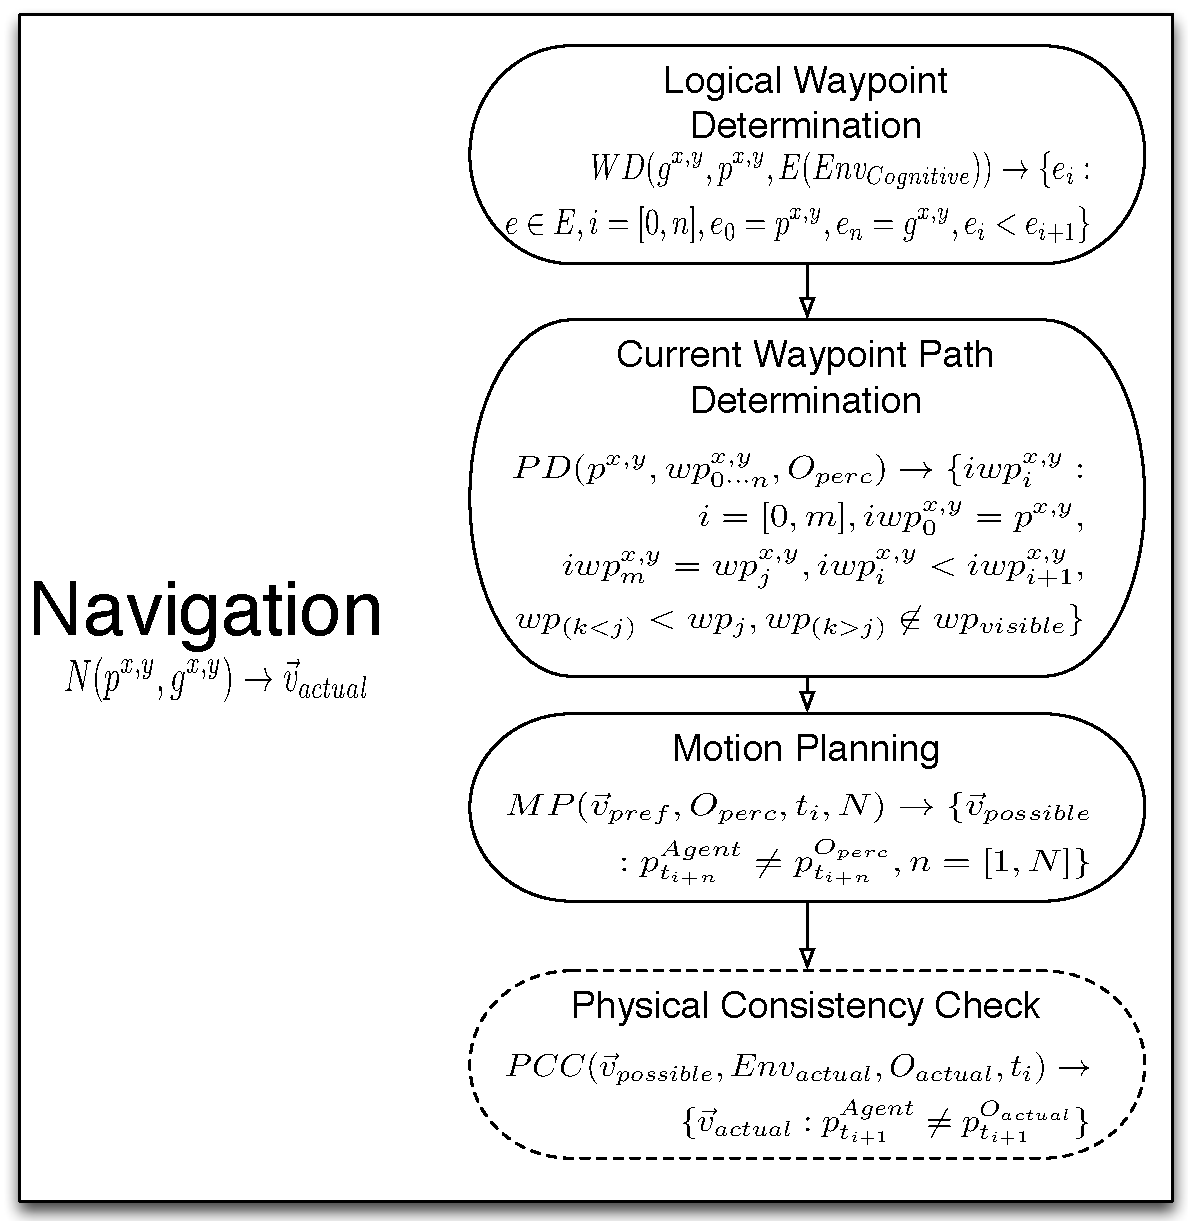
\includegraphics[height=5in]{NavigationWithFormula}
\caption[Detailed Navigation Model]{Mathematical depiction of the working of Navigation Model}
\label{fig:detailedNavigationModule}
\end{figure}

The goal position~($g^{x,y}$) is first received by the \emph{Logical Waypoint Determination}~($WD$) system which then uses a route finding algorithm like A-star or Djikstra's~\cite{Russel:1995wca} to find a set of logical waypoints~($E_i$) that will lead the agent from its current position($p^{x,y}$) to the goal position~($g^{x,y}$). The logical waypoints in the path so planned will be a list of links from the agent's cognitive map~($Env_{cognitive}$). This implies two things: Firstly, it looks at the environment at the room/ area level. Secondly, the agent plans a path according to his personal cognitive map hence there is no assurance that the path planned by two agents from the same point will be exactly the same. This step is called a waypoint determination step because it returns a set of logical waypoints to be used by the agent to reach its goal. This set of logical waypoints is then passed to the next level of navigation, i.e.\ \emph{the Current Waypoint Path Determination} step.

The \emph{Current Waypoint Path Determination}~($PD$) differs from the higher layer in that it takes into consideration dynamic obstacles i.e.\ other agents, as well as the static obstacles to determine a collision free path from the current location to the farthest visible waypoint. The logical waypoints are first converted to a set of concrete waypoints~($WP^{x,y}$) which are actual locations on the map. Using the set of perceived obstacles~($O_{perc}$) a set of intermediate waypoints~($IWP^{x,y}$) that would enable a collision free path to the farthest visible concrete waypoint~($wp^{x,y}_j$) is calculated and passed to the next level. This level can also be referred to as the \emph{strategic planning step} since it tries to model how a person strategically moves from one point to another while ensuring that it minimizes collisions with others. One possible way of doing this is by using a pattern based motion system~\cite{Nan:2011vr} or the effort minimizing algorithm ClearPath~\cite{Guy:2009gu}.

The preferred velocity of the agent is then set to velocity that would lead it to the next intermediate concrete waypoint determined by the PD. Ideally, this preferred velocity should ensure collision free motion. However, since the strategy is based on the prediction of the movement of dynamic agents who themselves use such dynamic planning it is inevitable that some collisions can happen if agents only follow their preferred velocities. Hence we use a lower level \emph{Motion Planning}~($MP$) which steps in, when necessary, to avoid collisions. There are several popular collision avoidance algorithms likes Reciprocal Velocity Obstacles~\cite{Guy:2010ko,Yeh:2008tg} and Social force~\cite{Helbing:1995ie} based methods. These were discussed in detail in Chapter~\ref{chapter:IBP}. At each time step~($t_i$), these algorithms take a preferred velocity~($\vec{v}_{pref}$) and set of obstacles~($O_{perc}$) (both static and dynamic) as input and output a possible velocity~($\vec{v}_{possible}$) that the agent can use to ensure that collisions do not occur for the next $N$ seconds. The two important points of difference from the previous layer is that it has some noticeable effect only when a collision is imminent and that it is very short term (limited to a few time steps) as compared to PD.

Since the Motion Planning system works on the basis of perceived obstacles and not actual obstacles, there is a chance, especially in dense environments, that the predicted velocity might cause a collision. In such cases, the lowest level \emph{Physical Consistency Check}~($PCC$) layer ensures that unnatural behavior is not produced. As the name suggests, this layer ensures that physical consistency is maintained and people don't walk through other people and static obstacles in the environment during the next time step~($t_{i+1}$). This is the only layer in the agent that uses the actual map($Env_{actual}$) and actual obstacles($O_{actual}$) instead of the personal cognitive map and perceived obstacles.

In summary, the Navigation Module receives a goal that is passed to the highest level which determines a high level route through the different areas in the environment to the goal; this waypoint is passed to the next level which determines a path towards the current waypoint that avoids dynamic obstacles and calculates a preferred velocity that the agent should take to follow this path; this preferred velocity is checked by the emergency collision avoidance mechanism to ensure that collisions are avoided and it returns a modified or unmodified actual velocity that is as close as possible to the preferred velocity and avoids collisions for the next time step of the simulation; and finally, the physical consistency check ensures that the simulation remains realistic by making sure that objects don't pass through each other.

\section{Summary}
\label{RemainingModulesSummar}

In the chapter, the design of the modules other than the IBP module has been discussed. First, the Event Knowledge Module was introduced. Besides, giving a brief review of the theoretical grounding of the model, the concept of \emph{buckets} and their thresholds for event identification was explained. Following this, the role of the ADM in defining an agent's individuality through its intrinsic features was explained along with the module's significance in the IBEVAC architecture. The Environment Knowledge Module's working was then explained after introducing relevant work on human cognitive maps. This was followed by an explanation of the proposed communication and planning modules. Finally, the navigation module's structure and working was explained with the help of a mathematical description. Each of these modules have been developed to different degrees. In the next and final chapter of this report, the extent of work remaining in model design, implementation and validation is presented along with a tentative schedule for completion of work on the thesis.